\section{Overview}

The software to be developed is a distributed application with a client-server multi-tiered architecture. \\
The general architecture of the system can be subdivided into the three logic layers:
\begin{itemize}
    \item \textit{Presentation Layer}: it handles the interaction with all kinds of user. It provides an interface to users accessing both the mobile application and the web application allowing them to exploit DREAM’s services in the most efficient and intuitive way. 
    \item \textit{Business logic or Application Layer}: it handles the functions to be provided for the users. It also manages communication between the end user interface and the database. 
    \item \textit{Data Layer}: it manages the persistent storage and retrieval of data accessing to the database. 
\end{itemize}

The three logic software layers are built on top of a four tier architecture, which consists in four different hardware tiers that represent a machine (or a group of machines):
\begin{itemize}
    \item \textit{Client tier}: it consists of the client programs that are used to exploit system’s services and the devices where those programs are installed, which in this case are pc for the web application and smartphone for the mobile applications.
    \item \textit{Web tier}: it consists of components that handle the interaction between client tier and the business tier. It contains Web Servers. It dynamically generates content in various formats for the client tier from which it collects inputs and return appropriate results from the components in the business tier.
    \item \textit{Business tier}: it processes all dynamic content and the interactions between the Client/Web Tier and the Data tier. It contains Application Servers.
    \item \textit{Data tier}: runs the DBMS and holds all of the sensitive application data. It contains database servers.
\end{itemize}

\begin{center}
    \begin{figure}[h!]
  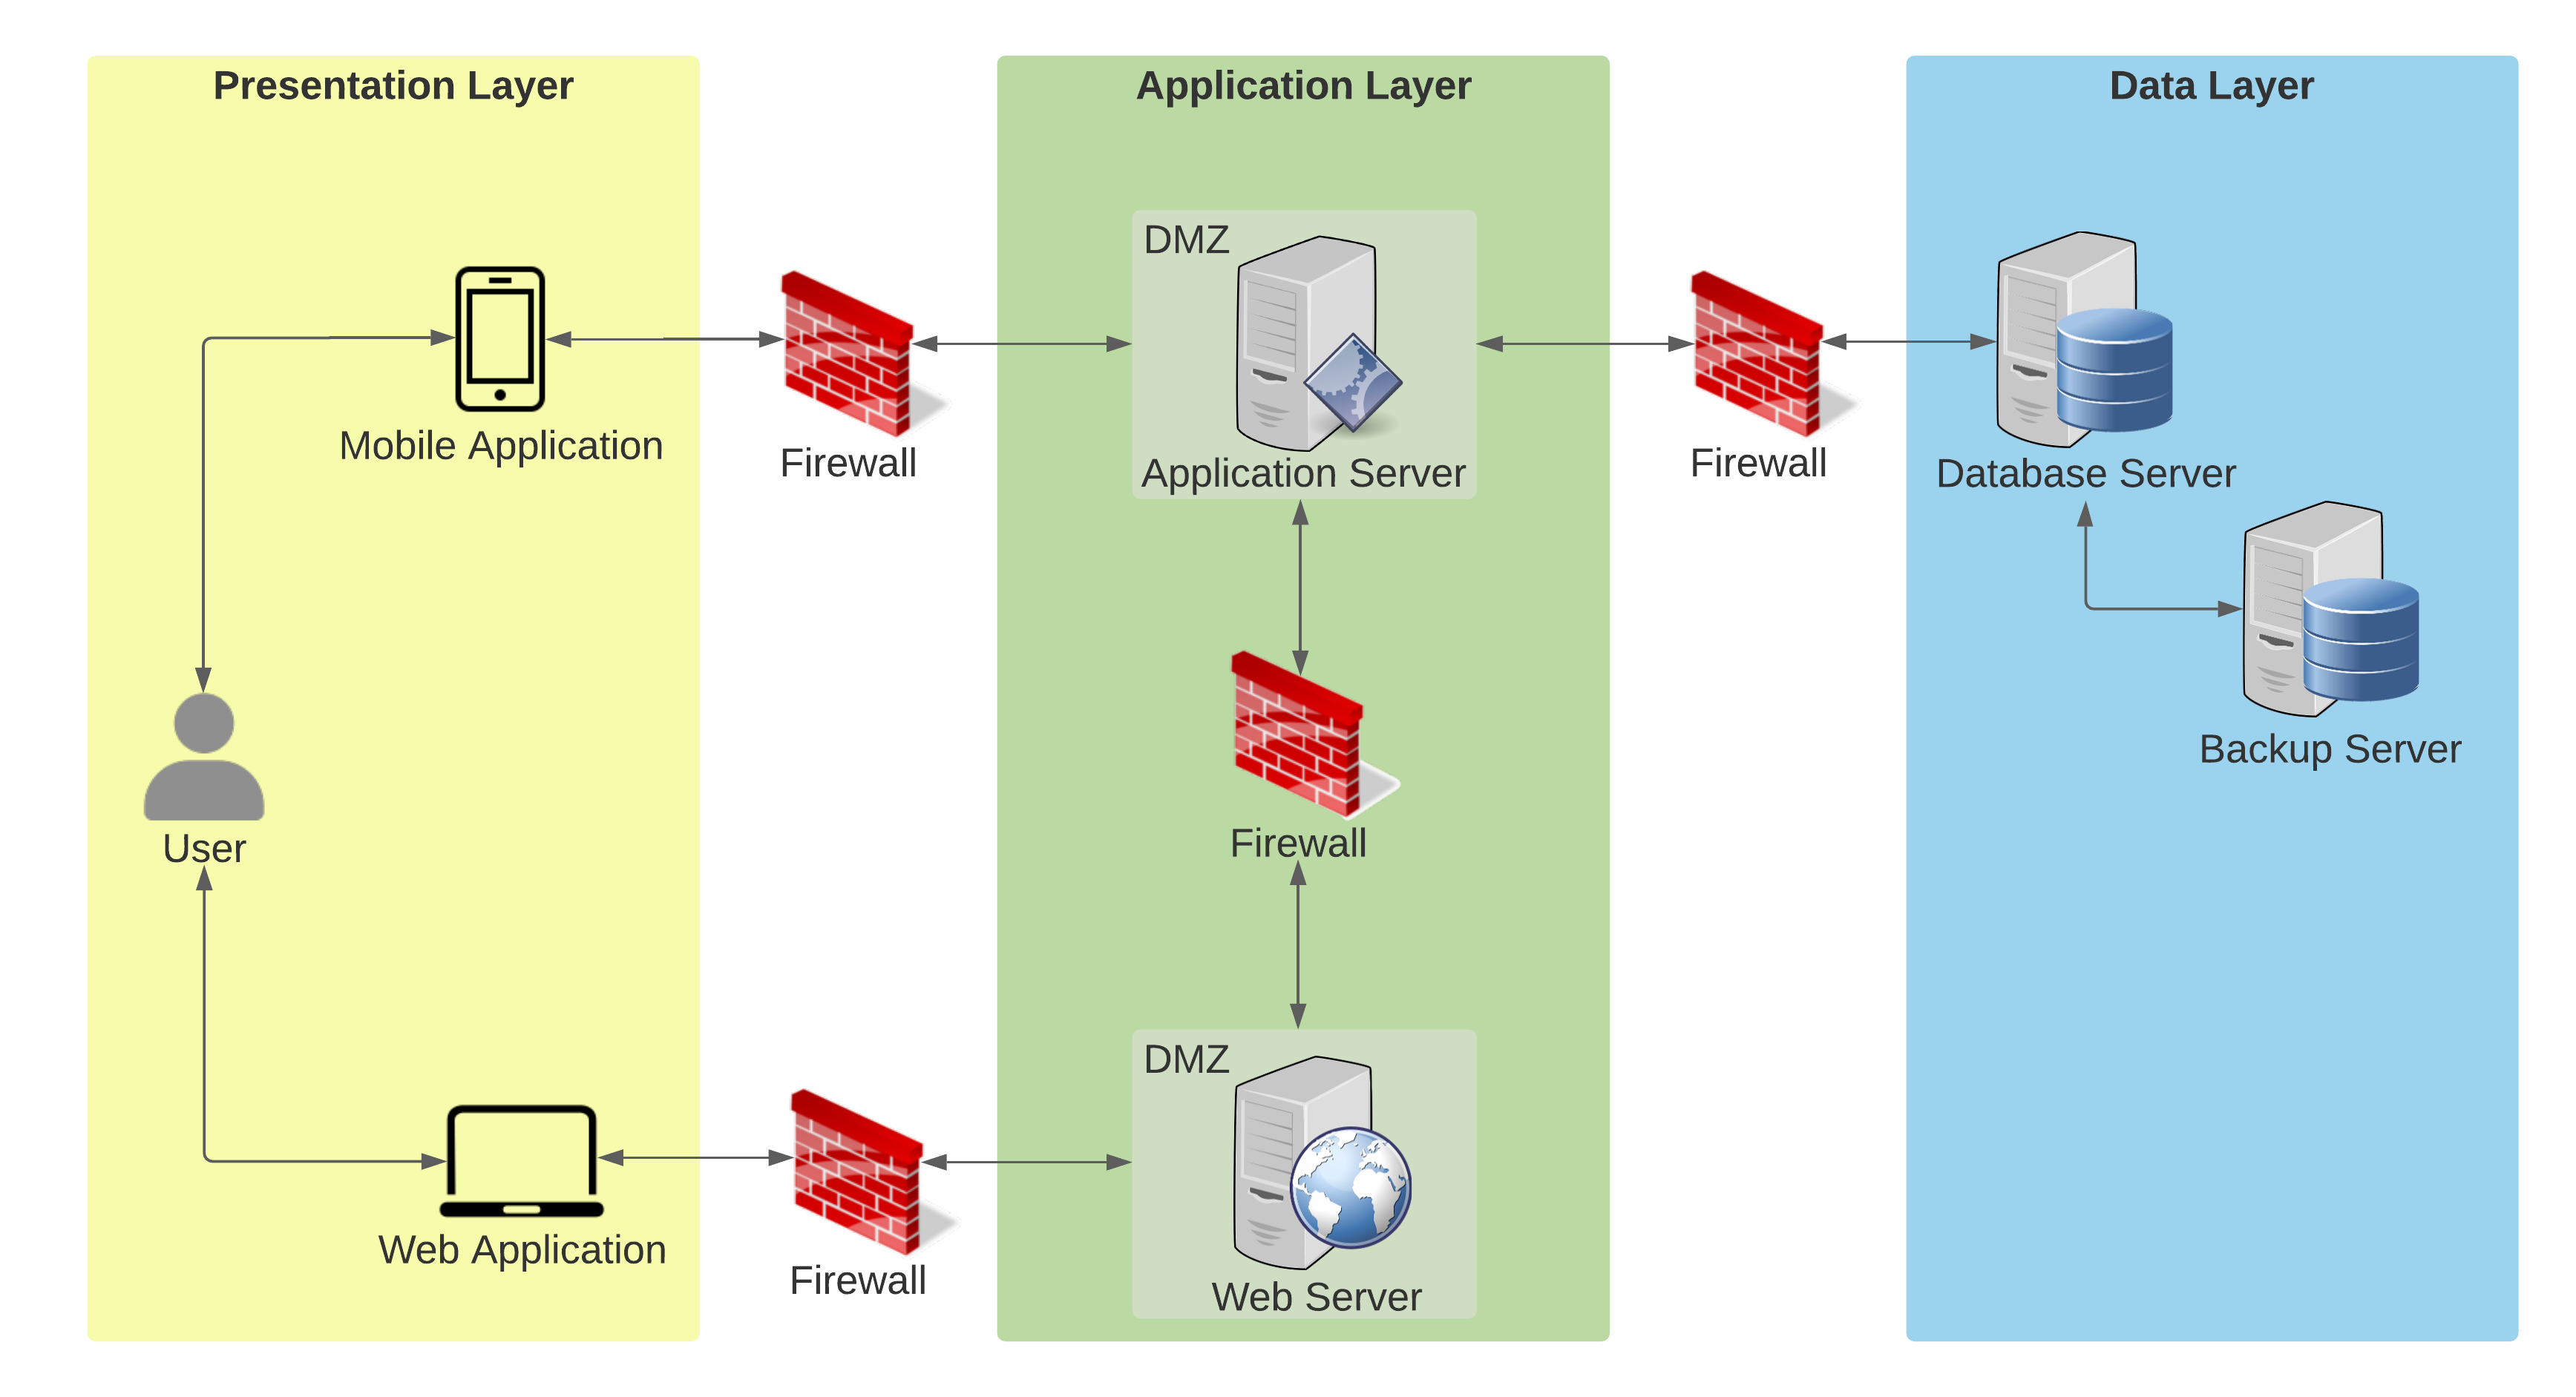
\includegraphics[width=\textwidth,height=\textheight,keepaspectratio]{./Images/System Architecture.png}
  \caption{System Architecture}
\end{figure}
\end{center}

The Application Server is the core of the system’s architecture as it is the central point between all the other components. It holds the business logic of the system with Web Server. Web and Application servers communicate to each other. It has persistent connection with Data tier and by communicating with its DBMS it can handle all the operations of reading, writing and uploading of data.\\

The service is supposed to be accessed through both a web application and a mobile application, and this is valid for all kinds of users. Users who access through DREAM web application can communicate with the Web Server while users logged into the mobile application communicate directly with the Application Server.\\

To guarantee high level of security due to the sensitivity of treated data, firewalls are installed before and after the Application tier to create a Demilitarized Zone (DMZ) for the application servers so that the external network can access only to the resources exposed in the DMZ. \\
Moreover, the Database Server periodically stores critical data in the Backup Server. \\

The described architecture has been chosen because tiering ensures the ability to scale applications, guaranteeing the system scalability and flexibility to future integrations and modifications.
The servers that constitute each tier in fact may differ both in capability and number. If needed, it can be possible to add more servers (horizontal scaling or scaling out) or more powerful servers (vertical scaling or scaling up) to each singular tier.  

\newpage